\documentclass{jsarticle}
\usepackage[dvipdfmx]{hyperref}
\usepackage[dvipdfmx]{graphicx}
\usepackage{amssymb,amsmath,amsthm}
\usepackage{listings,jlisting}
\usepackage{newtxtt}
\usepackage{cases}
\usepackage[utf8]{inputenc}

\date{\today}
\author{山田龍}
\title{}
\begin{document}
\maketitle
\section{課題1}
\subsection{ケース1}
まず、関数$f(t)$が、
\begin{numcases}
  {}
  -1 + 2t/\pi (0\leq t \leq \pi)& \\
  3 - 2t/\pi (\pi\leq t \leq 2\pi) &
\end{numcases}
と与えられるとき、フーリエ係数を解析的に求める。
フーリエ係数は、
\begin{align}
    c_k &= \frac{1}{T}\int f(t) e^{-i \frac{2 \pi kt}{T}}dt\\
    &= \frac{1}{2\pi}\int^{\pi}_{0}(-1 + 2t/\pi) e^{-ikt} dt
     + \frac{1}{2\pi}\int^{2\pi}_{\pi}(3 - 2t/\pi) e^{-ikt} dt\\
\end{align}
いま、$te^{-ikt}$の不定積分が
\begin{align}
    \int te^{-ikt} &= \left[ - \frac{te^{-ikt}}{ik}\right] + \int \frac{1}{ik}e^{-ikt}dt + C\\
         &= \left[ - \frac{te^{-ikt}}{ik}\right] + \frac{1}{k^2}\left[e^{-ikt}\right] + C\\
\end{align}
であることを使えば、
\begin{align}
    2\pi c_k &= \left[\frac{e^{-ikt}}{ik}\right]^{\pi}_0
    + \frac{2}{\pi}\left[ - \frac{te^{-ikt}}{ik}\right]^{\pi}_0
    + \frac{2}{\pi}\frac{1}{k^2}\left[e^{-ikt}\right]^{\pi}_0 
    - 3\left[\frac{e^{-ikt}}{ik}\right]^{2\pi}_{\pi}
    + \frac{2}{\pi}\left[\frac{te^{-ikt}}{ik}\right]^{2\pi}_{\pi}
    - \frac{2}{\pi}\frac{1}{k^2}\left[e^{-ikt}\right]^{2\pi}_{\pi}\\
    &= \frac{e^{-ik\pi} - 1}{ik}
    - \frac{2}{\pi}\frac{\pi e^{-ik\pi}}{ik}
    + \frac{2}{\pi}\frac{e^{-ik\pi} - 1}{k^2} 
    - 3\frac{e^{-ik2\pi} - e^{-ik\pi}}{ik}
    + \frac{2}{\pi}\frac{2\pi e^{-ik2\pi} - \pi e^{-ik\pi}}{ik}
    - \frac{2}{\pi}\frac{e^{-ik2\pi} - e^{-ik\pi}}{k^2}\\
    &= \frac{(-1)^k - 1}{ik}
    - 2\frac{(-1)^k}{ik}
    + \frac{2}{\pi}\frac{(-1)^k - 1}{k^2} 
    - 3\frac{1 - (-1)^k}{ik}
    + 2\frac{2 - (-1)^k}{ik}
    - \frac{2}{\pi}\frac{1 - (-1)^k}{k^2}\\
    &= \frac{2}{\pi}\frac{(-1)^k - 1}{k^2} 
    - \frac{2}{\pi}\frac{1 - (-1)^k}{k^2}\\
    &= \frac{2}{\pi k^2} ((-1)^k - 1 - 1 + (-1)^k)\\
    &= \frac{4}{\pi k^2} ((-1)^k - 1)\\
    \therefore c_k &= \frac{2}{\pi^2 k^2} ((-1)^k - 1)\label{eq:a1}
\end{align}
解析解が求められた。次に
\begin{equation}
    f_N(t) = \sum^N_{-N} c_k e^{ikt}
\end{equation}
を使って$f_N$を計算した結果を図示すると図\ref{f1}のようになる。
\begin{figure}[htbp]
    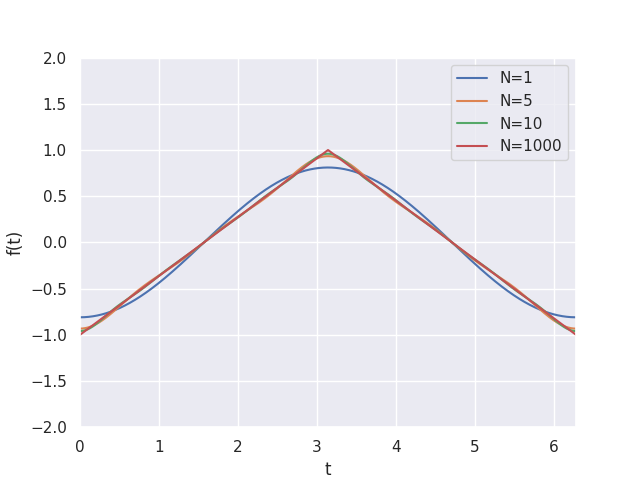
\includegraphics[clip,width=10.0cm]{./fourier_case1.png}
    \caption{$f_N$が$f(t)$の分布に近づく様子}
    \label{f1}
\end{figure}
また、誤差$f(t) - f_N(t)$の$N$依存性は図\ref{f2}のようになる。
この図から、誤差は$N$の増大とともに急激に消えることがわかる。
右側のプロットは両対数グラフであるが、傾きから$f(t) - f_N(T) \propto N^{-2}$であることがわかる。
\begin{figure}[htbp]
    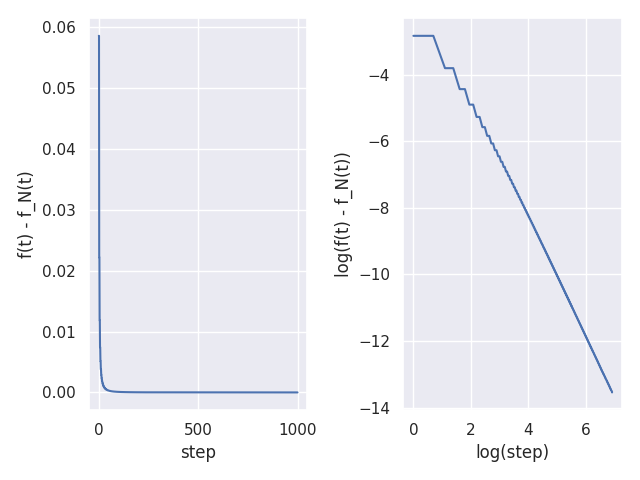
\includegraphics[clip,width=10.0cm]{./fourier_error_case1.png}
    \caption{誤差}
    \label{f2}
\end{figure}
\subsection{ケース2}
次に、関数$f(t)$が、
\begin{numcases}
  {}
  1 (0\leq t \leq \pi)& \\
  -1 (\pi\leq t \leq 2\pi) &
\end{numcases}
と与えられるとき、フーリエ係数を解析的に求める。
フーリエ係数は、
\begin{align}
    c_k &= \frac{1}{T}\int f(t) e^{-i \frac{2 \pi kt}{T}}dt\\
    &= \frac{1}{2\pi}\int^{\pi}_{0}e^{-ikt} dt
     + \frac{1}{2\pi}\int^{2\pi}_{\pi}-e^{-ikt} dt\\
\end{align}
\begin{align}
    2\pi c_k &= - \left[\frac{e^{-ikt}}{ik}\right]^{\pi}_0 
    + \left[\frac{e^{-ikt}}{ik}\right]^{2\pi}_{\pi}\\
    &= \frac{2}{ik} (-(-1)^k + 1)\\
    \therefore c_k &= \frac{1}{i\pi k} (-(-1)^k + 1)
\end{align}
したがって、$c_k$は$k$が偶数のとき$0$で、奇数のとき
\begin{equation}
    c_k = \frac{2}{i\pi k}
\end{equation}
解析解が求められた。次に
\begin{equation}
    f_N(t) = \sum^{N}_{k=-N} c_k e^{ikt}
\end{equation}
を具体的に書き下せば、
\begin{align}
    f_N(t) &= \sum^{\lfloor \frac{n+1}{2}\rfloor}_{m=1}
    \frac{4}{\pi k}\left( \frac{e^{ikt} - e^{-ikt}}{2i}\right) (k = 2m -1)\\
    &= \sum^{\lfloor \frac{n+1}{2}\rfloor}_{m=1}
    \frac{4}{\pi k}\sin(kt) (k = 2m -1)\\
    &= \sum^{\lfloor \frac{n+1}{2}\rfloor}_{m=1}
    \frac{4}{\pi (2m-1)}\sin((2m-1)t)\label{eq:statement}
\end{align}
$f_N$を計算した結果を図示すると図\ref{f3}のようになる。$t=0$付近でギブス不連続が見られる。
そしてそのピークでは$y=1.18$である。
\begin{figure}[htbp]
    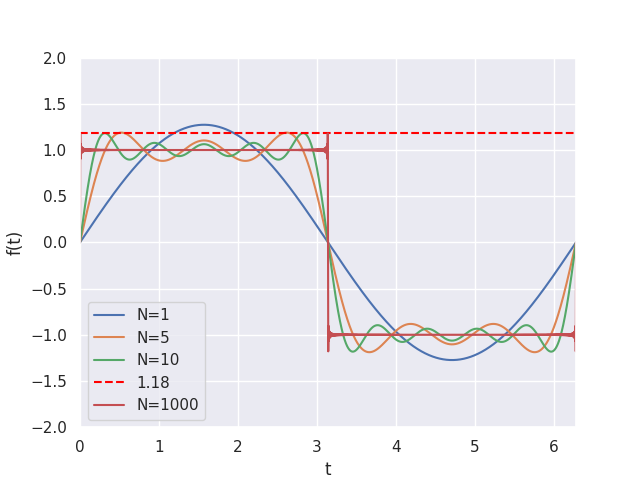
\includegraphics[clip,width=10.0cm]{./fourier_case2.png}
    \caption{$f_N$が$f(t)$の分布に近づく様子}
    \label{f3}
\end{figure}
また、誤差$f(t) - f_N(t)$の$N$依存性は図\ref{f4}のようになる。
この図から、誤差は$N$の増大とともに急激に消えることがわかる。
右側のプロットは両対数グラフであるが、傾きから$f(t) - f_N(T) \propto N^{-1}$であることがわかる。
\begin{figure}[htbp]
    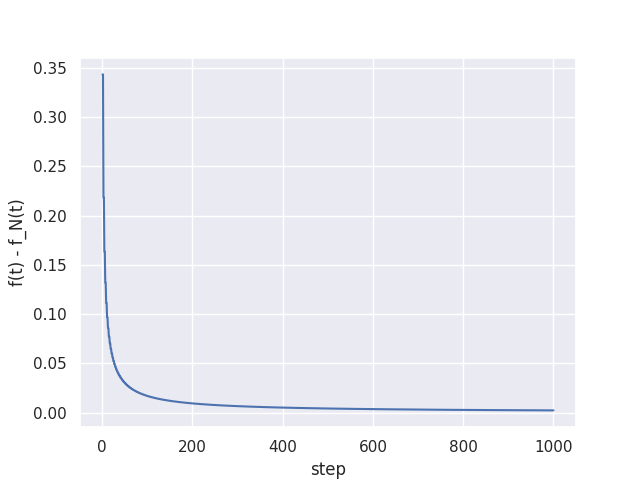
\includegraphics[clip,width=10.0cm]{./fourier_error_case2.png}
    \caption{誤差}
    \label{f4}
\end{figure}
\subsection{ギブス不連続}
\eqref{eq:statement}を使ってギブス不連続について考える。
ギブス不連続の$t=0$近傍でのピークでは、$f(t)$の一階導関数が$0$になると考えられる。
\begin{align}
    f'(t)&= \sum^{\lfloor \frac{n+1}{2}\rfloor}_{m=1}
    \frac{4}{\pi}\cos((2m-1)t)\\
    &= \frac{4}{\pi}\sum^{\lfloor \frac{n+1}{2}\rfloor}_{m=1}
    \cos((2m-1)t)\\
\end{align}
ここで、三角関数の位相の等差数列はチェビシェフ多項式の計算のように複素指数関数の等比数列に変形すれば計算できる。
したがって、$M=\lfloor \frac{n+1}{2}\rfloor$として、
\begin{align}
    f'(t)&= \frac{4}{\pi}\sum^{M}_{m=1}
    Re\left(e^{i(2m-1)t}\right)\\
    &= \frac{4}{\pi}\sum^{M}_{m=1}
    Re\left(e^{i(2m-1)t}\right)\\
    &= \frac{4}{\pi}
    Re\left(e^{it}\frac{1 - e^{2iMt}}{1 - e^{2it}}\right)\\
    &= \frac{4}{\pi}
    Re\left(e^{it}\frac{1 - e^{2iMt}}{1 - e^{2it}}\frac{1 - e^{-2it}}{1 - e^{-2it}}\right)\\
    &= \frac{4}{\pi}
    Re\left((e^{it} - e^{-it})\frac{1 - e^{2iMt}}{2 - e^{2it}- e^{-2it}}\right)\\
    &= \frac{4}{\pi}
    Re\left((2i\sin(t))\frac{1 - e^{2iMt}}{2 - 2\cos(2t)}\right)\\
    &= \frac{4}{\pi}
    Re\left((i\sin(t))\frac{1 - e^{2iMt}}{2\sin^2t}\right)\\
    &= \frac{4}{\pi}
    Re\left(i\frac{1 - e^{2iMt}}{2\sin t}\right)\\
    &= \frac{4}{\pi}\frac{1}{2\sin t}
    Re\left(i(1 - e^{2iMt})\right)\\
    &= \frac{2}{\pi}\frac{1}{\sin t}
    Re\left(i(1 - \cos (2Mt) -i \sin (2Mt))\right)\\
    &= \frac{2}{\pi}\frac{\sin (2Mt)}{\sin t} = 0\\
\end{align}
を解けば、$\sin (2Mt) = 0$より$t_p = \frac{\pi}{2M}$がピークである。
ピークでの$f(t_p)$の値は、
\begin{align}
    f(t_p) &= f(0) + \int^{t_p}_0 f'(x) dx\\
    &= \frac{2}{\pi}\int^{t_p}_0 \frac{\sin (2Mx)}{\sin x} dx\\
    &= \frac{2}{\pi}\int^{t_p}_0 \sin (2Mx)\left(\frac{1}{\sin x} - \frac{1}{x} + \frac{1}{x}\right) dx\\
    &= \frac{2}{\pi}\int^{t_p}_0 
    \sin (2Mx)
    \left(\frac{1}{\sin } - \frac{1}{x}\right) dx
    +\frac{2}{\pi}\int^{t_p}_0 
    \frac{\sin (2Mx)}{x} dx\\
    &= I_1 + I_2
\end{align}
第一項を$I_1$、第二項を$I_2$と置く。
$y = \frac{1}{\sin x} - \frac{1}{x}$は$[0, \frac{\pi}{2}]$で
\begin{equation}
    0 \leq \frac{1}{\sin x} - \frac{1}{x} \leq \frac{2(\pi - 2)}{\pi} x
\end{equation}
が成立する。したがって、
\begin{equation}
    I_1 \leq \int^{t_p}_0 \frac{2(\pi - 2)}{\pi} x dx = \frac{\pi - 2}{\pi}t_p^2 
\end{equation}
であるから、$n \rightarrow \infty$で$I_1 \rightarrow 0$であることがわかる。
したがって、
\begin{align}
    f(t_p) &= \frac{2}{\pi}\int^{t_p}_0 
    \frac{\sin (2Mx)}{x} dx\\
    &= \frac{2}{\pi}\int^{\pi}_0 
    \frac{\sin (y)}{y} dy (y \rightarrow 2Mx)\\
\end{align}
この積分は正弦積分であり、
\begin{align}
    f(t_p) &= \frac{2}{\pi} 1.85193705\cdots\\
    &= 1.178979\cdots
\end{align}
ピークは$1.18$付近であることがわかった。
この節の解析は参考\cite{gibbs}に大きく依る。

\section{課題2}
作成したプログラムでは
\begin{equation}
    \hat{c}_k = \frac{1}{N}\sum^{N-1}_{n=0} f_n e^{-i2\pi kn/N}
\end{equation}
を使ってフーリエ係数計算し、
\begin{equation}
    f_n = \frac{1}{N}\sum^{N-1}_{n=0} \hat{c}_k e^{-i2\pi kn/N}
\end{equation}
よりデータ列を復元した。
関数$f(t)$
\begin{numcases}
  {}
  -1 + 2t/\pi (0\leq t \leq \pi)& \\
  3 - 2t/\pi (\pi\leq t \leq 2\pi) &
\end{numcases}
が与えられたとき、フーリエ係数の解析解は\eqref{eq:a1}であることがわかる。
ここで解析解と計算によって得た係数の誤差は、図\ref{f5}となる。
また、離散フーリエ変換にかかる時間を計測した結果が図\ref{f6}となる。
$t = O(N^2)$であることが傾きからわかる。
\begin{figure}[htbp]
    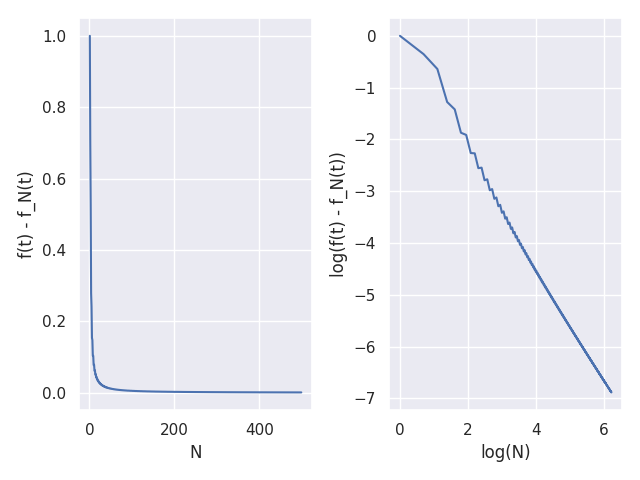
\includegraphics[clip,width=10.0cm]{./dft_error.png}
    \caption{DFTの誤差}
    \label{f5}
\end{figure}
\begin{figure}[htbp]
    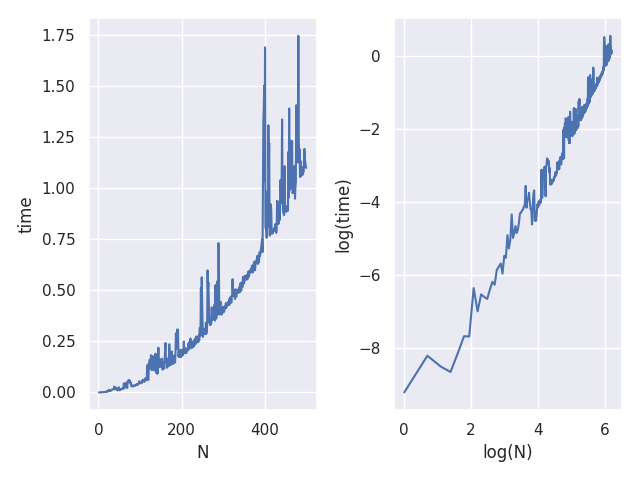
\includegraphics[clip,width=10.0cm]{./dft_time.png}
    \caption{DFTの処理時間}
    \label{f6}
\end{figure}

\section{課題3}
\begin{equation}
    f(t) = \sin(t) + \sin(\sqrt{2}t)
\end{equation}
からデータ列を作成して、離散フーリエ変換を実行したあとパワースペクトルを計算する。
結果は図\ref{f7}のようになる。
サンプリング数を増やすとピークが鋭くなり、裾が小さくなる。
\begin{figure}[htbp]
    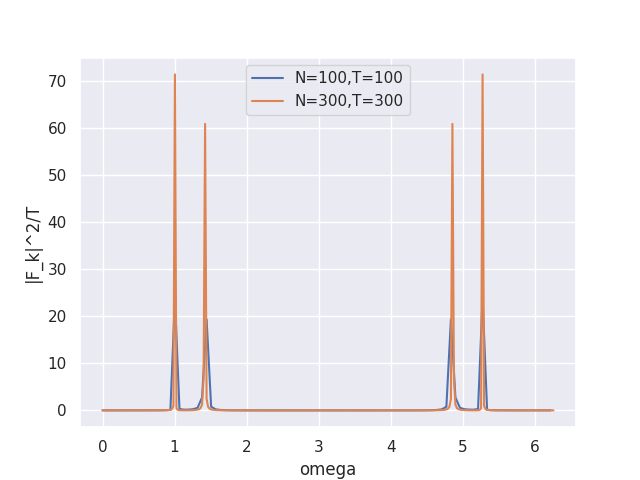
\includegraphics[clip,width=10.0cm]{./power.png}
    \caption{Power Spectral}
    \label{f7}
\end{figure}
\section{プログラム}
全て\href{https://github.com/tychy/NumericalAnalysisPlayground}{https://github.com/tychy/NumericalAnalysisPlayground}にあります。
\bibliographystyle{junsrt}
\bibliography{cite}
\end{document}